\section{Contiki Overview}

\subsection{Network Overview}

\begin{figure}[H]
	\centering
	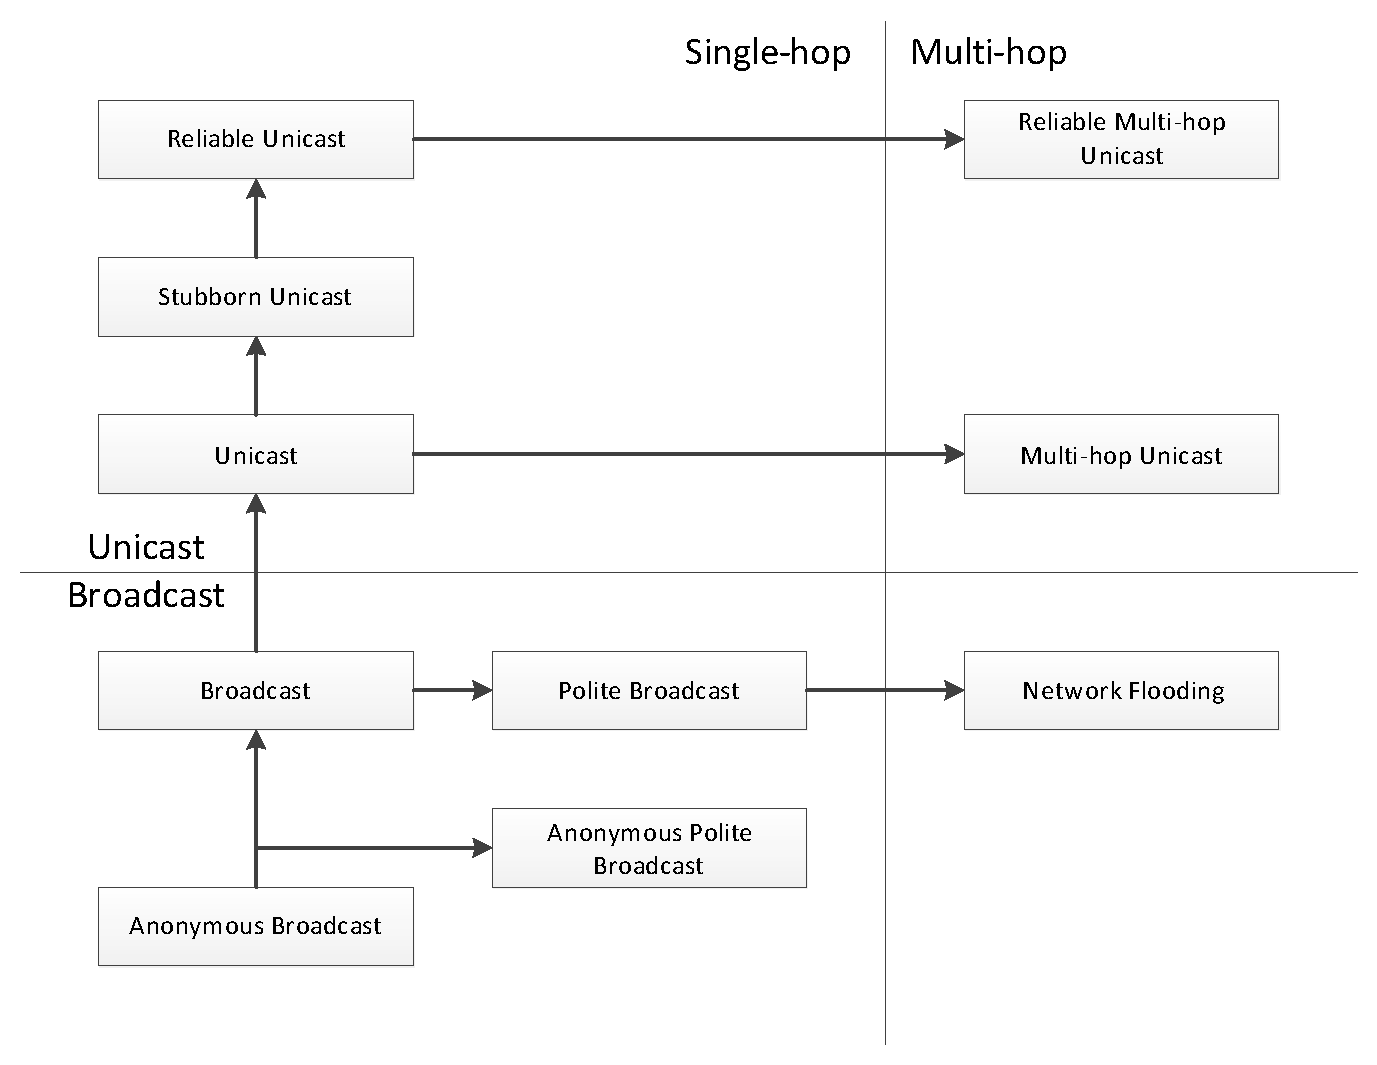
\includegraphics[width=\textwidth]{Diagrams/rime-stack}
	\caption{The communication primitives in the Rime network stack \cite{Dunkels:2007:ACA:1322263.1322295}}
\end{figure}

\subsubsection{Anonymous Broadcast}

\subsubsection{Broadcast}

\subsubsection{Anonymous Polite Broadcast}

\subsubsection{Polite Broadcast}

\subsubsection{Unicast}

\subsubsection{Stubborn Unicast}

\subsubsection{Reliable Unicast}

\subsubsection{Network Flooding}

\subsubsection{Multi-hop Unicast}

\subsubsection{Reliable Multi-hop Unicast}



\subsection{Network Channels}

Channels in Contiki are virtual \cite{tel-aviv-contiki-exercises}. This means that when a connection is opened if you do not want to receive packets from another connection then a different channel should be used. It does not mean that different radio frequencies are used. To use different radio frequencies the function \verb|cc2420_set_channel| should be used to change the frequency messages are broadcasted on.
